\documentclass{article}

\usepackage[utf8]{inputenc}
\usepackage[T1]{fontenc}
\usepackage{geometry}
\usepackage{graphicx}
\usepackage{subcaption}
\usepackage{verbatim}
\usepackage{amsmath,amssymb}
\geometry{a4paper}

\usepackage[french,italian]{babel}
\frenchspacing

\title{Relazione dell'esperimento del reticolo olografico}
\author{Lorenzo Ramella}
\date{13 gennaio 2021}

\begin{document}
\maketitle

\begin{abstract}
L’esperimento si propone di usare un reticolo olografico di passo noto per misurare le lunghezze d'onda di alcune lampade di uso quotidiano. I risultati ottenuti sono stati quindi usati per stimare il passo di un secondo reticolo olografico.

L'esperimento si è svolto in un ambiente domestico con strumenti di fortuna.

L'esperimento si è concluso con i seguenti risultati:

\vspace{4mm}

\begin{center}
\begin{tabular}{ || c | c | c | c || }
  \hline
  $\lambda (m)$ & $blu$ & $verde$ & $rosso$ \\
  \hline \hline &&& \\ [-0.9ex]
  lampada $1$ & $4,510 \cdot 10^{-7}$ & $5,43 \cdot 10^{-7}$ & $6,68 \cdot 10^{-7}$ \\
  $\sigma$ & $8 \cdot 10^{-10}$ & $2 \cdot 10^{-9}$ & $3 \cdot 10^{-9}$ \\
  lampada $2$ & $4,623 \cdot 10^{-7}$ & $5,57 \cdot 10^{-7}$ & \\
  $\sigma$ & $1,3 \cdot 10^{-9}$ & $2 \cdot 10^{-9}$ & \\
  \hline
\end{tabular}
\end{center}

\vspace{4mm}

La mia miglior stima del passo del secondo reticolo è:

\[9,3 \cdot 10^{-7} \pm 3 \cdot 10^{-8} \; \textrm{m}\]

\end{abstract}
\tableofcontents

\clearpage

\section{Introduzione teorica}

La luce che raggiunge un reticolo viene diffratta secondo la legge 

\begin{equation}
d(\textrm{sin} \, \phi_m (\lambda) + \textrm{sin} \, \theta) = m\lambda
\end{equation}

dove $\phi _m (\lambda)$ è l'angolo di diffrazione, in funzione della lunghezza d'onda e dell'ordine $m$, e $\theta$ è l'angolo di incidenza.

Nel caso $\theta = 0$

\begin{equation}
d(\textrm{sin} \, \phi_m (\lambda)) = m\lambda
\end{equation}

In particolare al primo ordine

\begin{equation}
\textrm{sin} \, \phi (\lambda) = \lambda/d
\end{equation}

Con questa formula è possibile misurare la lunghezza d'onda della luce incidente, se si ha a disposizione un reticolo di passo noto.

\vspace{5mm}

Ma come porsi nel caso $\theta = 0$ in ambiente domestico? È possibile nel caso in cui ci sia una distanza $z$ sufficientemente grande tra il reticolo e la sorgente di luce. Disponendo quindi un ''occhio'' (sia questo un occhio umano o un obiettivo di una fotocamera) dietro al reticolo, è sufficiente posizionare il reticolo ortogonalmente alla retta congiungente l'occhio e la fonte di luce. Se $z$ è sufficientemente grande, si possono quindi assumere i raggi incidenti sul reticolo come paralleli tra di loro e ortognali al reticolo.

\begin{figure}[h!]
  \centering
  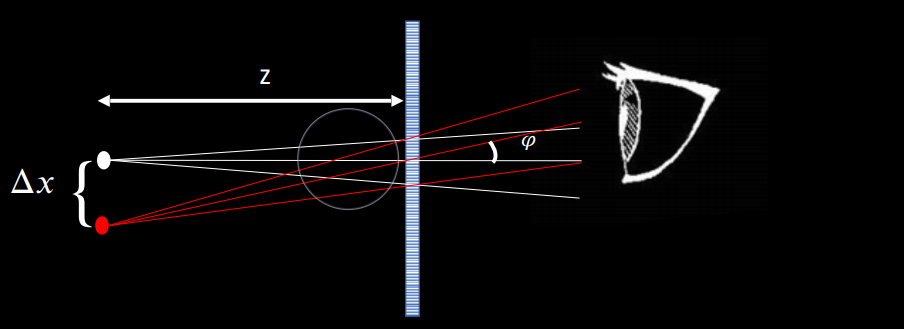
\includegraphics[width=0.8\linewidth]{IM_schema_1}
  \caption{Schema dell'esperimento}
  \label{schema}
\end{figure}

A questo punto l'occhio vede un'immagine diffratta (vedi Figura \ref{schema}) della sorgente luminosa (che per $z$ grande si può considerare puntiforme) che si trova ad una distanza 

\[\Delta x = z\, \textrm{tan} \, \phi\]

dalla sorgente luminosa. Per il primo ordine si possono assumere angoli $\phi$ piccoli, e si può usare l'approssimazione

\[\textrm{sin} \, \phi =\textrm{tan} \, \phi\]

da cui 

\begin{equation}
\Delta x = z\, \textrm{sin} \, \phi = \frac{z \cdot \lambda}{d}
\end{equation}

\section{Progettazione dell'esperimento}

\subsection{Lampada}

Per questo esperimento sono state usate due sorgenti luminose, d'ora in poi dette ``lampade'':

\begin{itemize}
  \item Lampada 1 è la torcia LED di uno smartphone, incastrato in un portapenne cilindrico di raggio $4$ cm (misurato con un comune righello, $s = 1 \; \textrm{mm}$).
  \item Lampada 2 è una comune torcia LED
\end{itemize}

\begin{figure}[h]
  \centering
  \begin{subfigure}[b]{0.4\linewidth}
    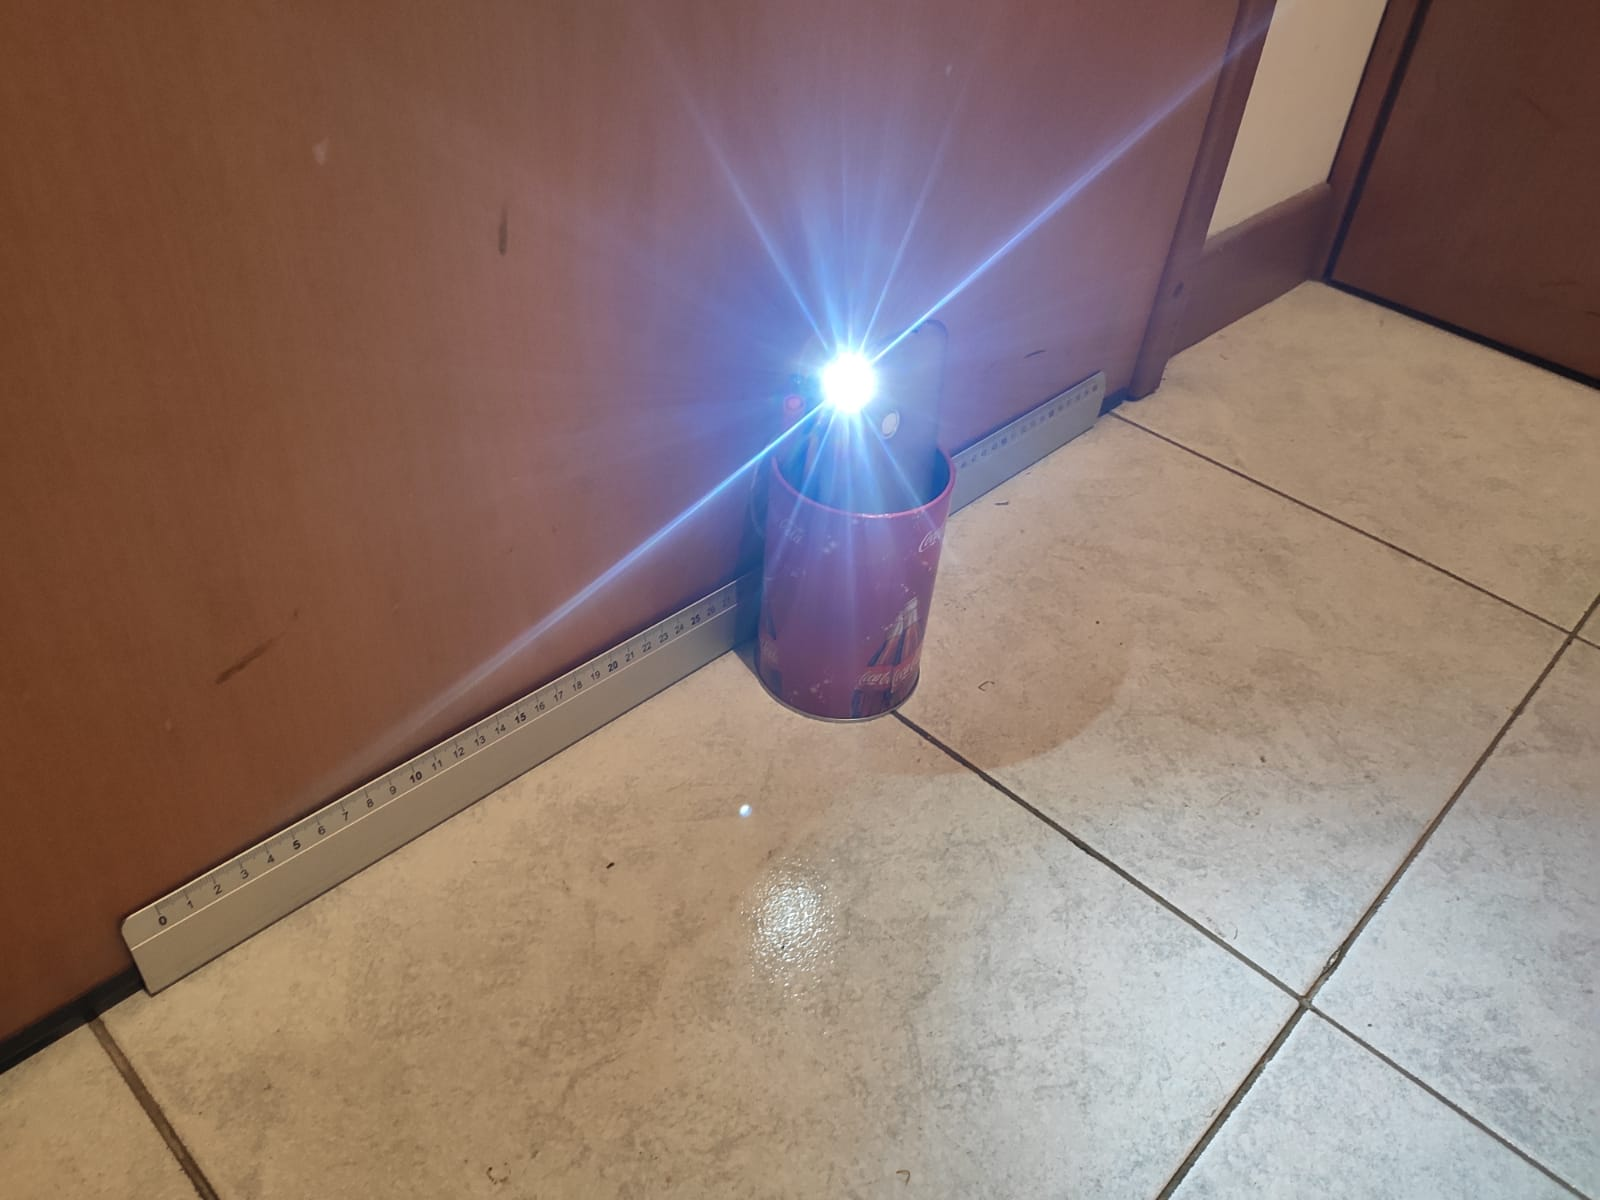
\includegraphics[width=\linewidth]{IM_foto_lamp_1}
    \caption{Foto della lampada 1}
  \end{subfigure}
  \begin{subfigure}[b]{0.4\linewidth}
    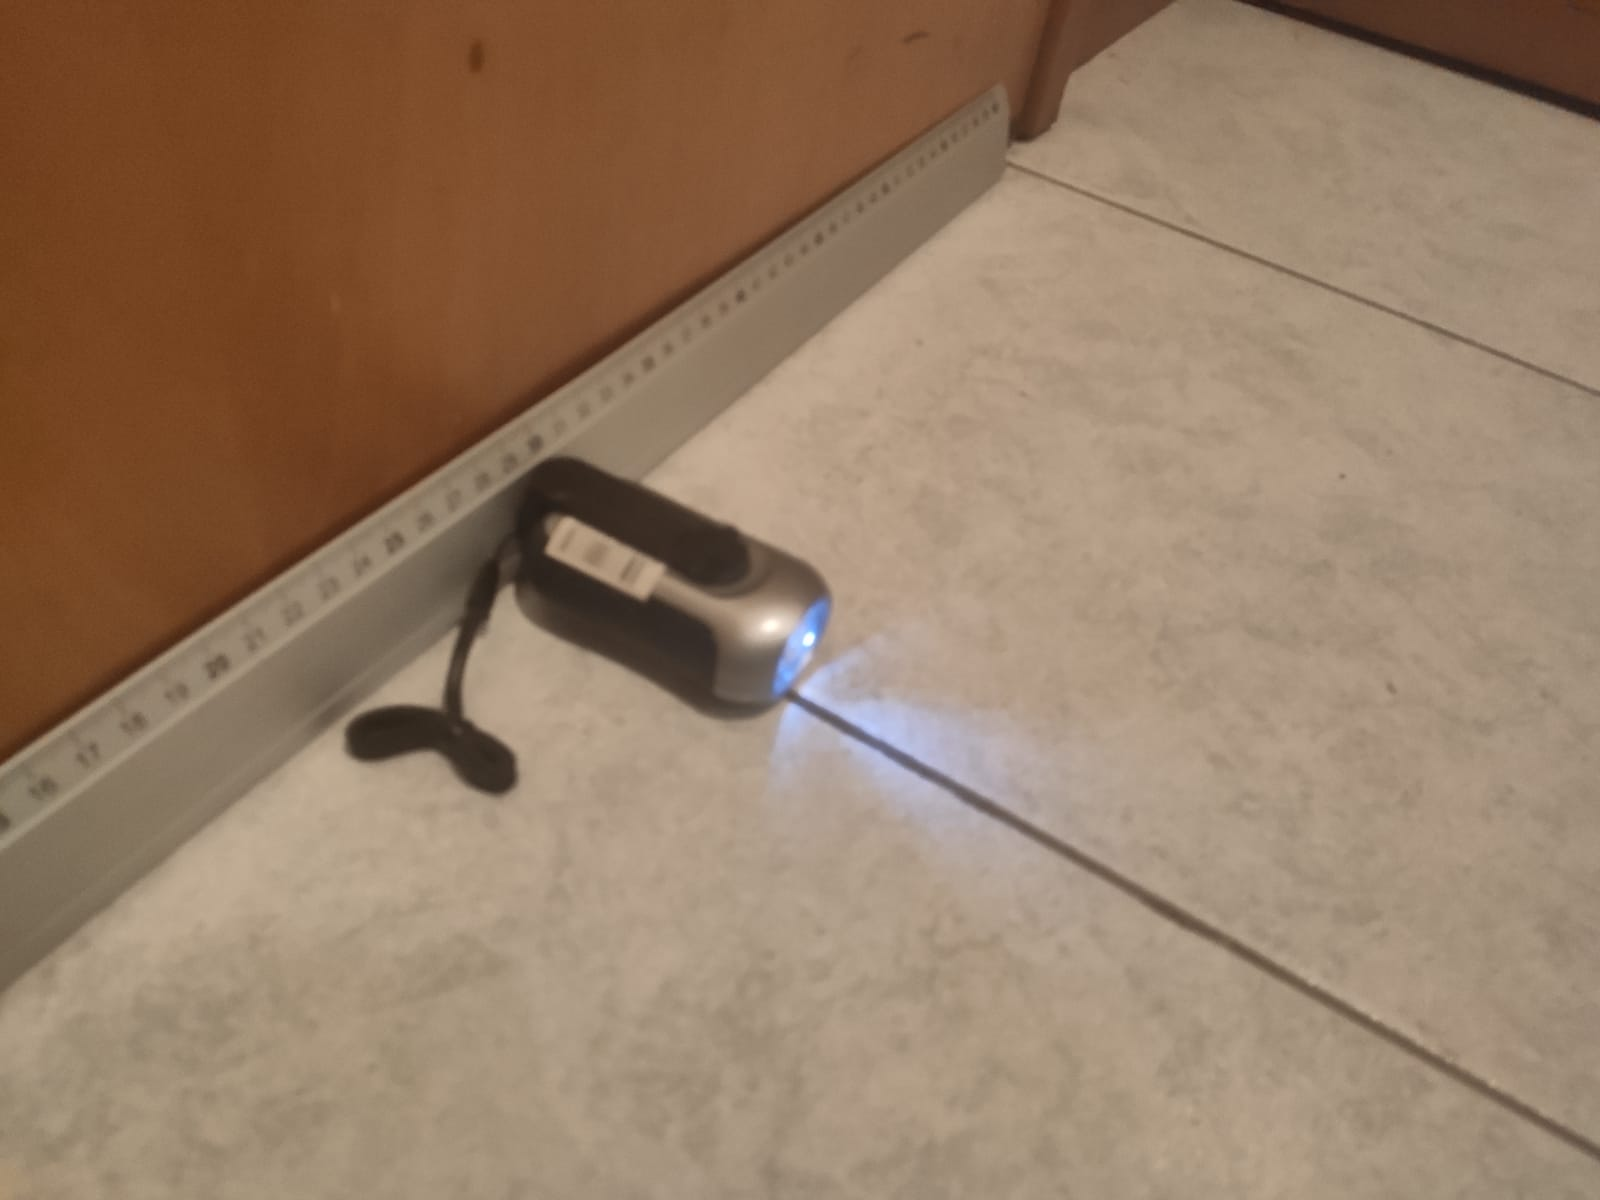
\includegraphics[width=\linewidth]{IM_foto_lamp_2}
    \caption{Foto della lampada 2}
  \end{subfigure}
  \caption{Foto delle lampade usate per l'esperimento}
\end{figure}

Durante la misura, le lampade sono state poste a ridosso della porta, lungo la linea di congiunzione tra due piastrelle (dettaglio importante per l'ortogonalizzazione). Una riga di metallo, lunga 62 cm, è stata posta a ridosso della porta. Questa tornerà utile in fase di analisi dati.

\subsection{Occhio}

\begin{figure}[h]
  \centering
  \begin{subfigure}[b]{0.4\linewidth}
    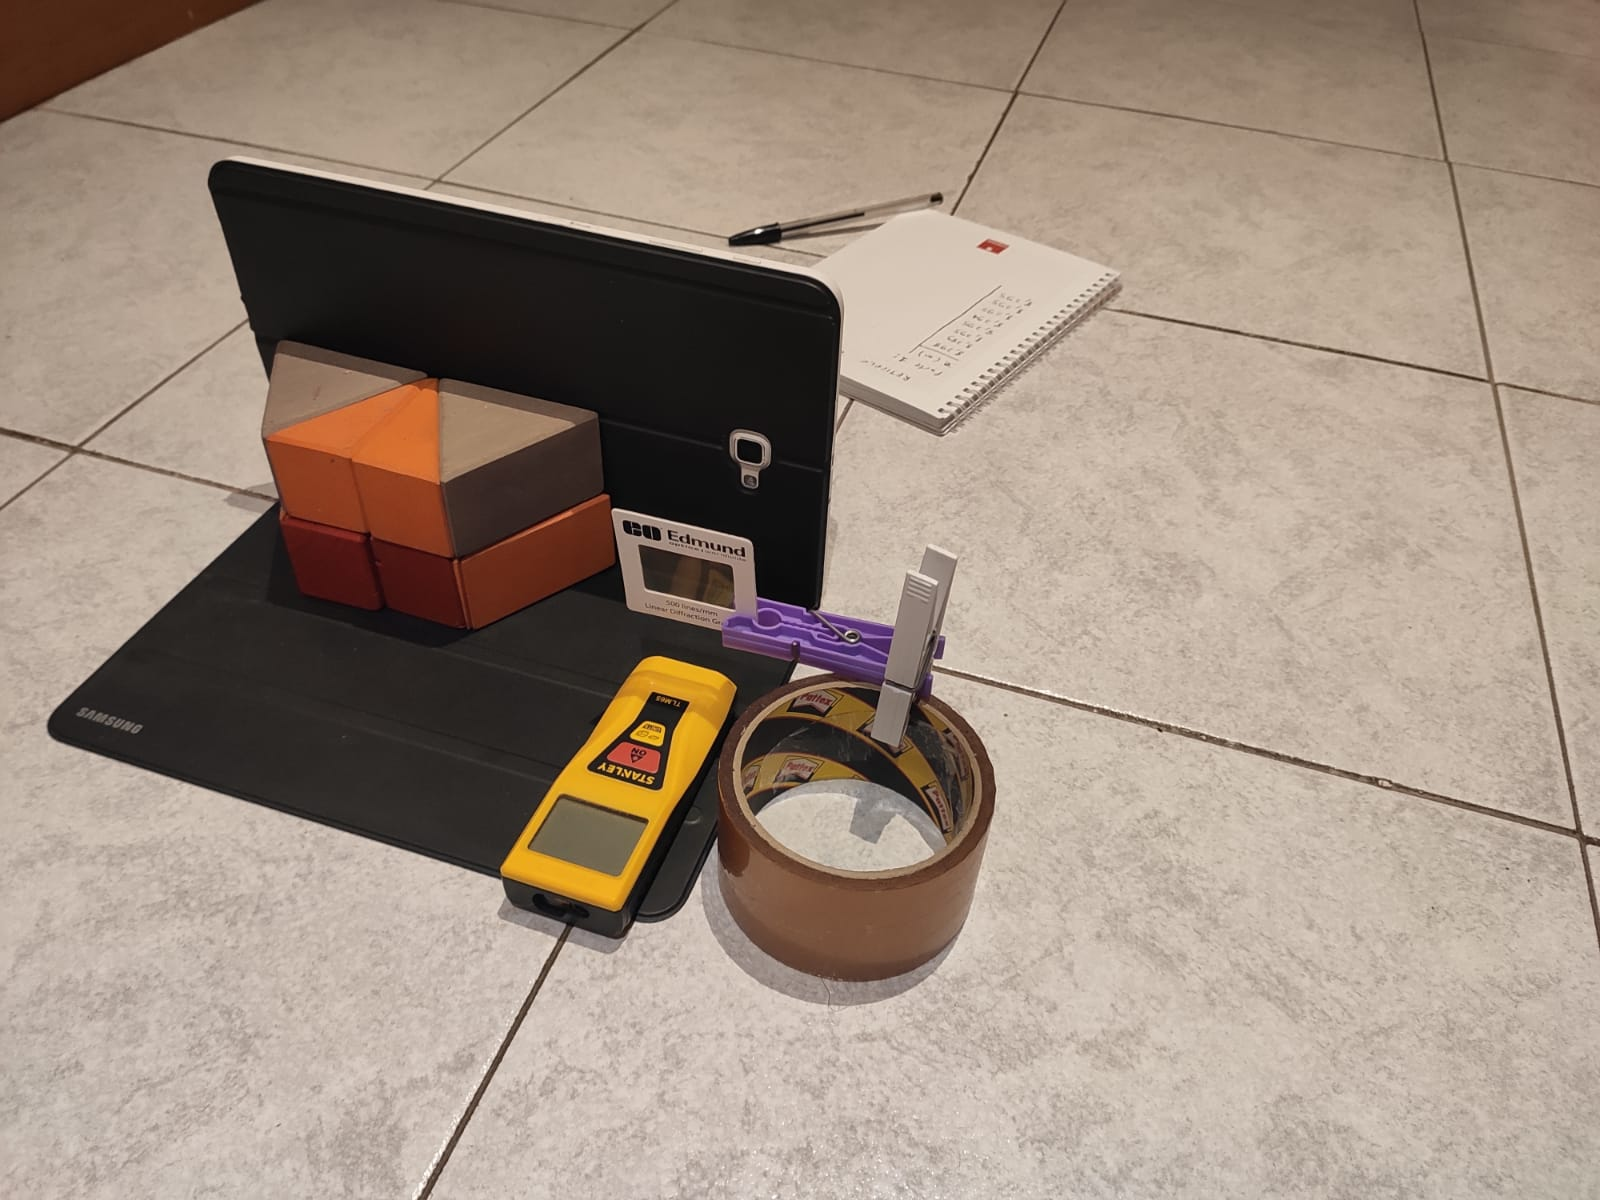
\includegraphics[width=\linewidth]{IM_foto_occhio_1}
  \end{subfigure}
  \begin{subfigure}[b]{0.4\linewidth}
    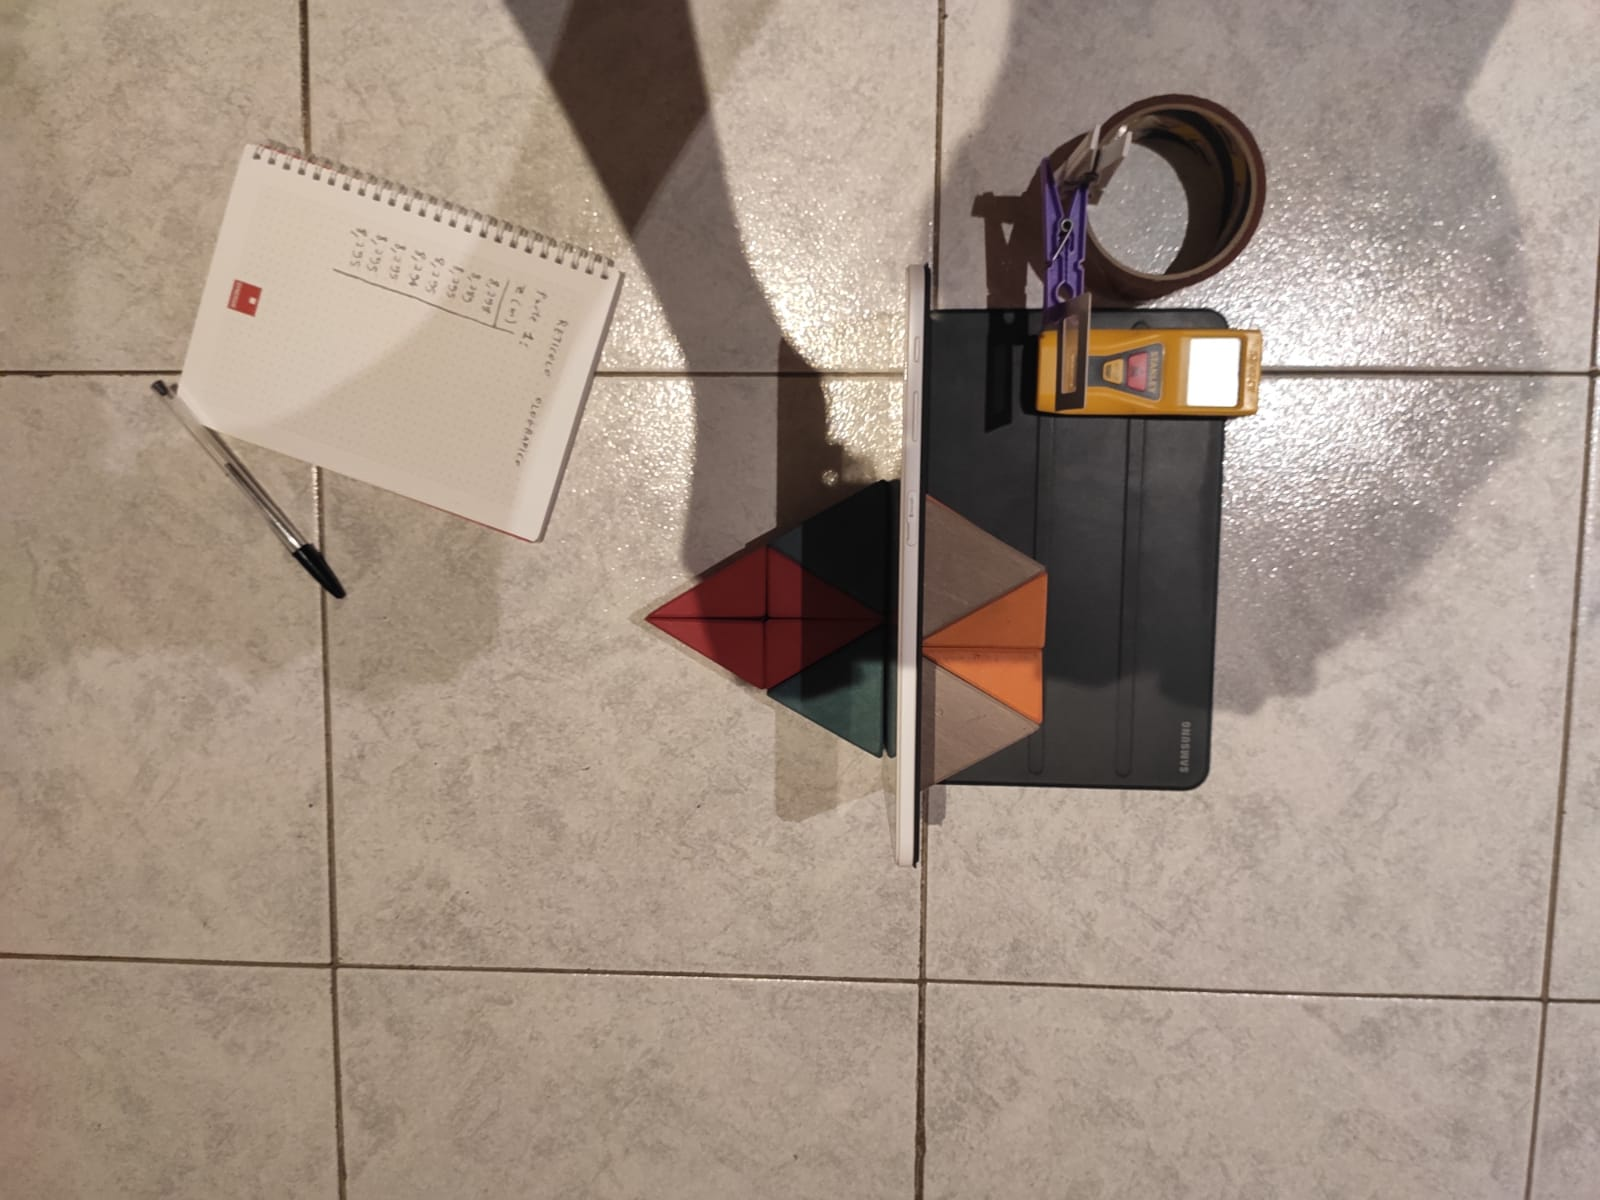
\includegraphics[width=\linewidth]{IM_foto_occhio_2}
  \end{subfigure}
  \caption{Foto dell'occhio}
\end{figure}

L' ``occhio'' è la struttura con cui sono state scattate le foto della sorgente luminosa e della sua immagine diffratta. Un tablet, tenuto in posizione verticale da dei mattoncini di legno, è posizionato in modo tale da avere la fotocamera posizionata approssimativamente lungo la stessa linea di congiunzione delle piastrelle della lampada. Le linee di congiunzione ad essa perpendicolari sono state usate per posizionare il tablet parallelamente alla porta.

\vspace{5mm}

Il reticolo è tenuto in posizione verticale da un supporto, costituito da un nastro di scotch e da delle mollette. Usando come riferimento le linee della piastrellatura, è stato angolato in modo tale da essere il più possibile ortogonale al raggio di luce incidente. Il reticolo di passo noto ha una densità dichiarata di $500$ righe/mm, che equivalgono ad un passo di circa $2 \cdot 10^{-6}$ m.

\vspace{5mm}

La distanza $z$ tra il reticolo e la fonte di luce è stata misurata usando un metro laser (sensibilità del millimetro).

\subsection{Misura di $\Delta x$}

Una volta fotografate le immagini, è stato usato un software di nome FIJI per la loro analisi. Usando come riferimento la riga metallica di lunghezza nota, sono state fatte le misure della distanza tra la sorgente luminosa e l'immagine diffratta per tutte le lunghezze d'onda visibili al primo ordine. Ogni misura è stata ripetuta quattro volte ed è stata fatta la media aritmetica, con la deviazione standard come incertezza. 

\section{Misure}

\subsection{lampada 1, reticolo passo noto}

Di questa lampada sono state fatte due misure, a due distanze diverse:

la prima a circa 8 metri di distanza, per avere come riferimento un valore di $z$ molto grande; 

la seconda, vista l'impraticità della misura ad 8 metri, è stata fatta a circa 3 metri di distanza.

\vspace{5mm}

Per la misura di $z$ sono state eseguite 8 misurazioni con il metro laser, mirando al centro del portapenne, e la deviazione standard è stata assunta come incertezza. Al valore finale è stato aggiunto un fattore di correzione di $9$ cm, dovuto al raggio di $4$ cm del portapenne e all'avvicinamento, in fase di misura, del reticolo alla fotocamera di $5$ cm (misurati con un comune righello, $s = 1$ mm) a causa di un iniziale posizionamento errato del reticolo (errore commesso in entrambe le misure a causa di una svista).

\vspace{5mm}

Di questa correzione ne è stato tenuto conto nell'incertezza nel seguente modo:

\[\sigma z = \sqrt{ \sigma^2 + 2\cdot s^2}\]

A questo punto è stato ricavata l'espressione di $\lambda$ partendo dalla Formula 4, e la relativa incertezza con la formula della propagazione degli errori:

\[\lambda = \frac{d \cdot \Delta x}{z} \quad \quad \quad \sigma \lambda = \sqrt{\left( \frac{d}{z} \sigma \Delta x \right)^2 + \left( -\frac{d \cdot \Delta x}{z^2}\sigma z \right)^2}\]

\begin{table}
\centering
\begin{tabular}{ | c | c | }
  \hline
  $\#$ & $z (m)$ \\
  \hline
  $1$ & $8,298$ \\
  $2$ & $8,289$ \\
  $3$ & $8,295$ \\
  $4$ & $8,295$ \\
  $5$ & $8,294$ \\
  $6$ & $8,295$ \\
  $7$ & $8,295$ \\
  $8$ & $8,295$ \\
  \hline 
  media & $8,295$ \\
  st. dev. & $0,002$ \\
  \hline
  $z$ (m) & $8,385$ \\
  $\sigma z$ (m) & $0,003$ \\
  \hline
\end{tabular}
\caption{Misura di $z$ (3.1, 8m)}
\end{table}

\begin{figure}[h!]
  \centering
  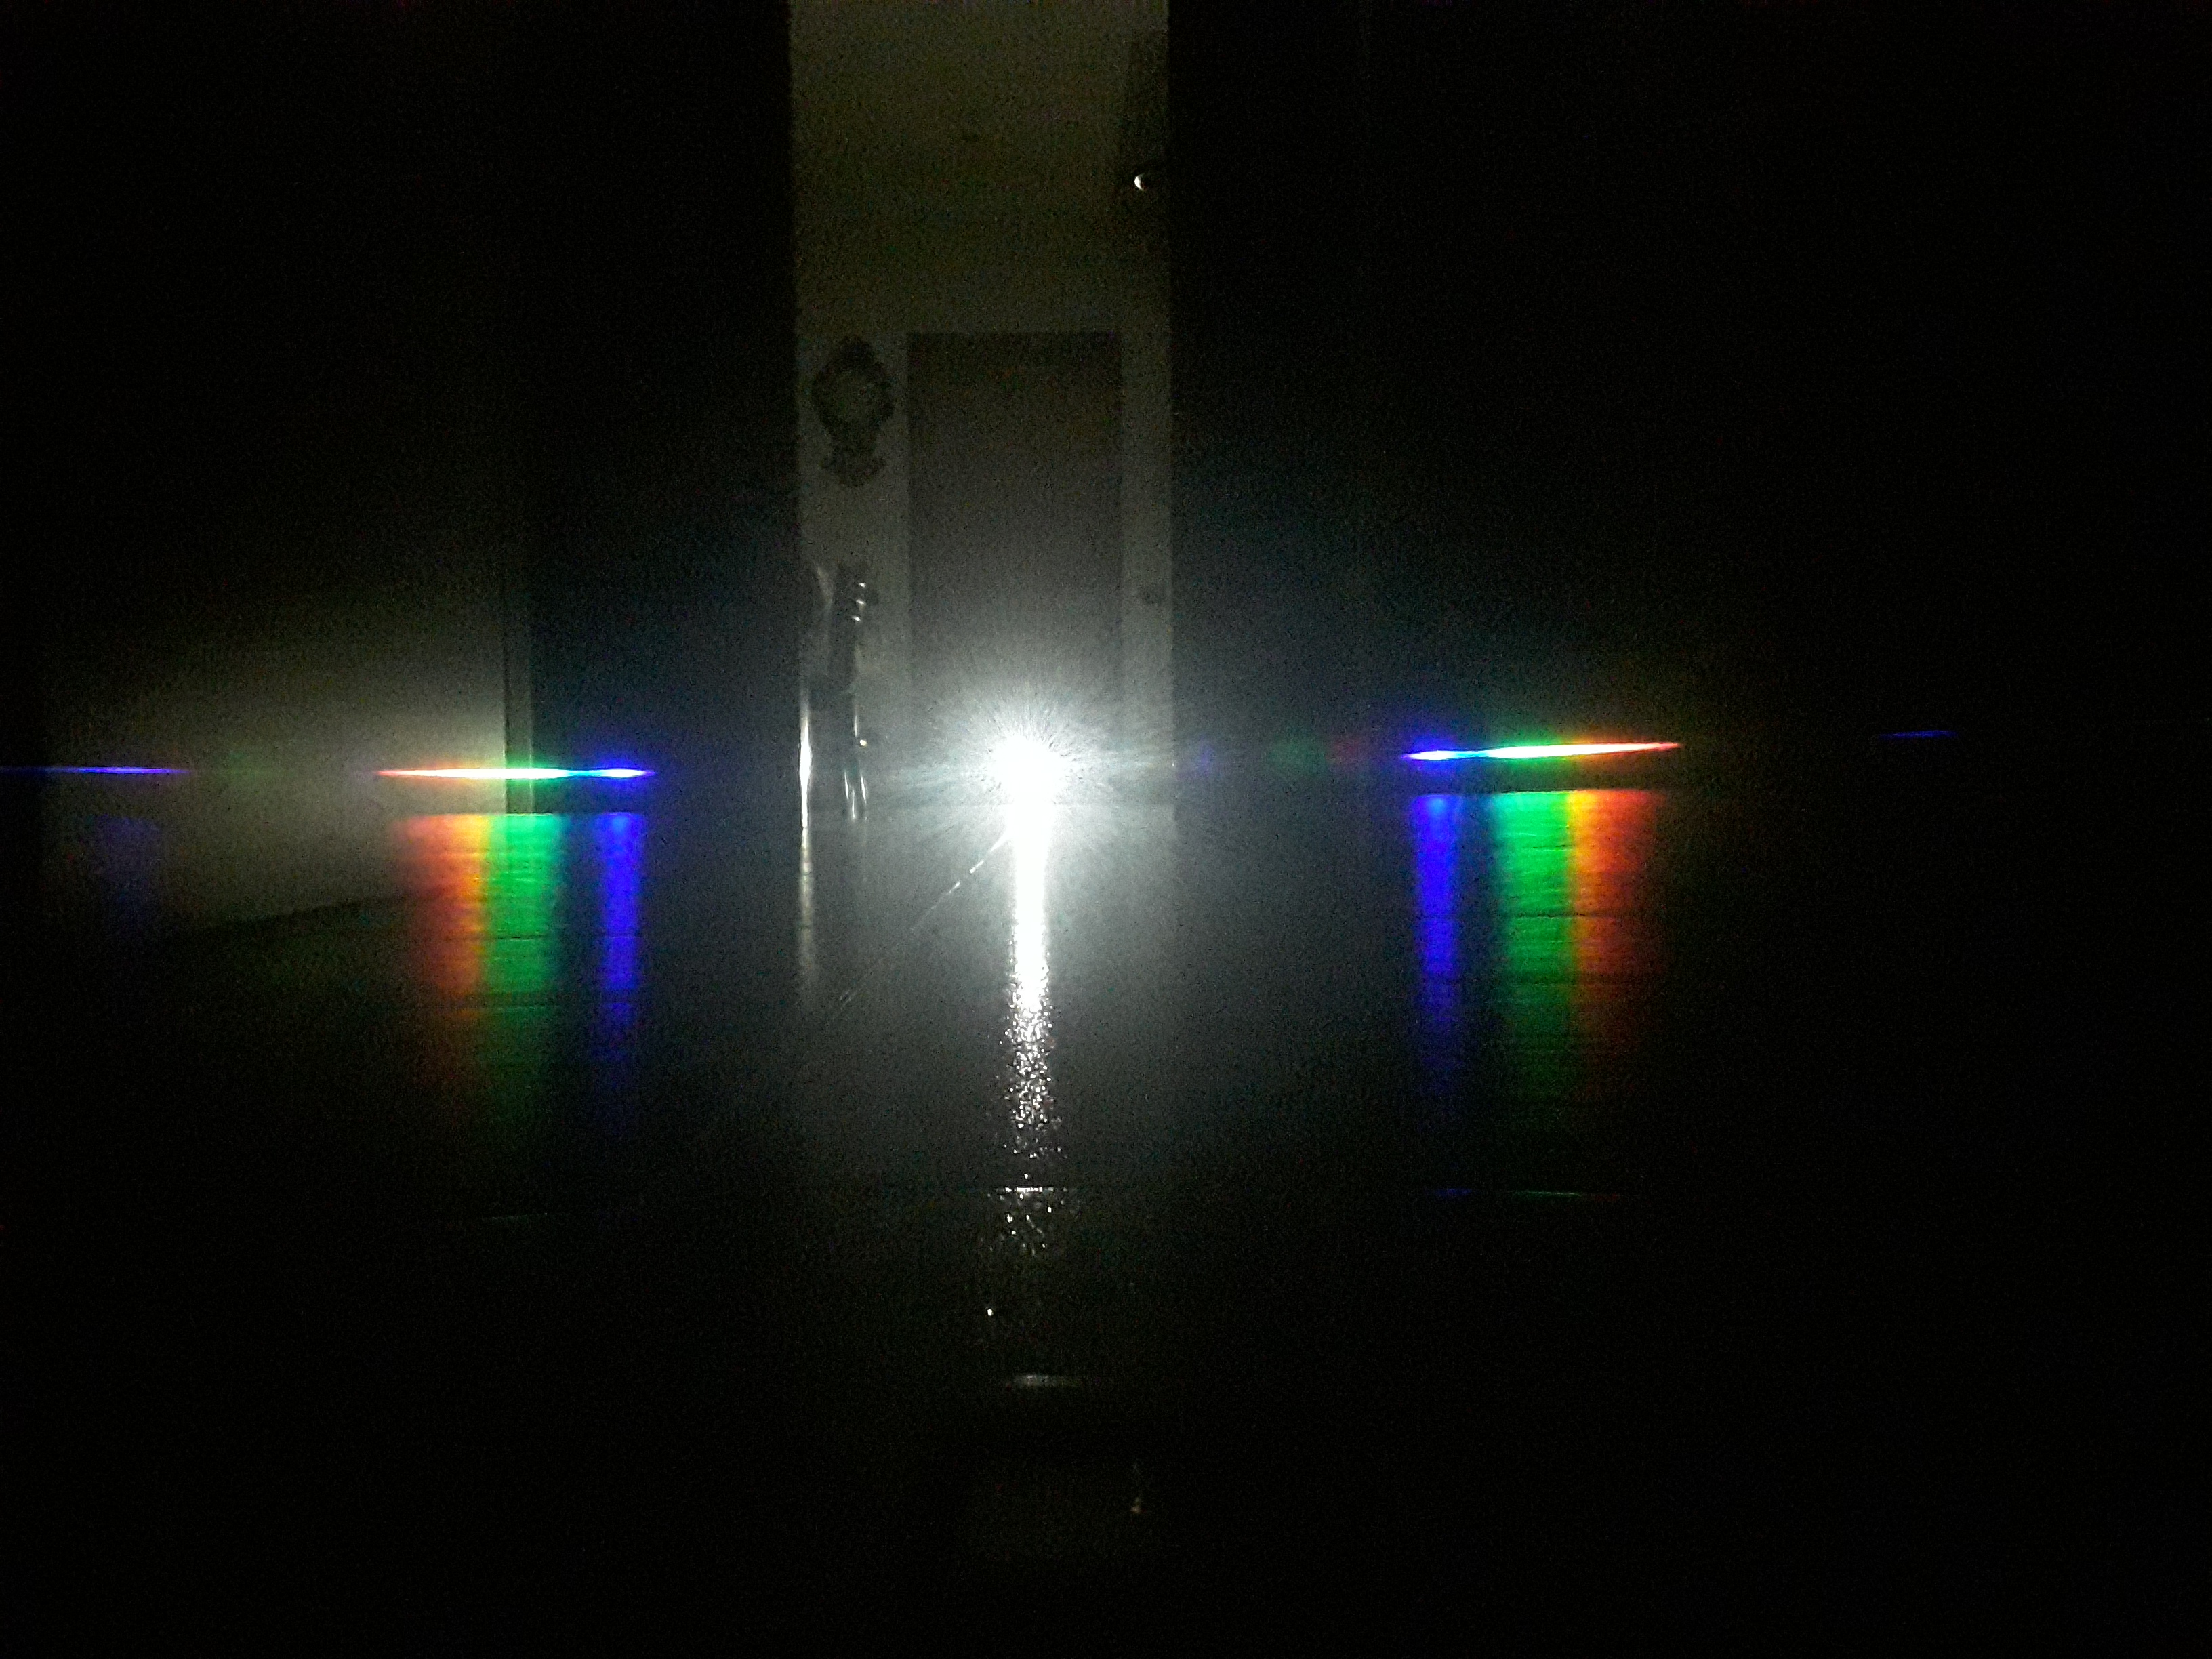
\includegraphics[width=0.6\linewidth]{IM 1.1.1}
  \caption{Foto della sorgente e dell'immagine diffratta (3.1, 8m)}
\end{figure}

\begin{figure}[h!]
  \centering
  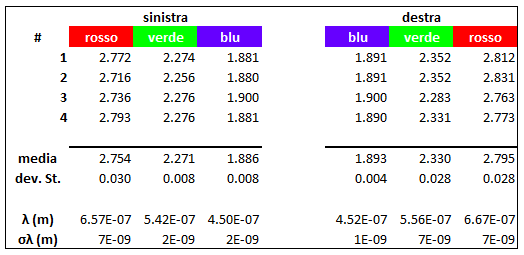
\includegraphics[width=0.6\linewidth]{IM tab_1.1.1}
  \caption{$\Delta x$ misurati (3.1, 8m)}
\end{figure}

\pagebreak

\begin{table}
\centering
\begin{tabular}{ | c | c | }
  \hline
  $\#$ & $z (m)$ \\
  \hline
  $1$ & $3,175$ \\
  $2$ & $3,178$ \\
  $3$ & $3,188$ \\
  $4$ & $3,175$ \\
  $5$ & $3,176$ \\
  $6$ & $3,176$ \\
  $7$ & $3,172$ \\
  $8$ & $3,173$ \\
  \hline 
  media & $3,177$ \\
  st. dev. & $0,005$ \\
  \hline
  $z$ (m) & $3,267$ \\
  $\sigma z$ (m) & $0,005$ \\
  \hline
\end{tabular}
\caption{Misura di $z$ (3.1, 3m)}
\end{table}

\begin{figure}[h!]
  \centering
  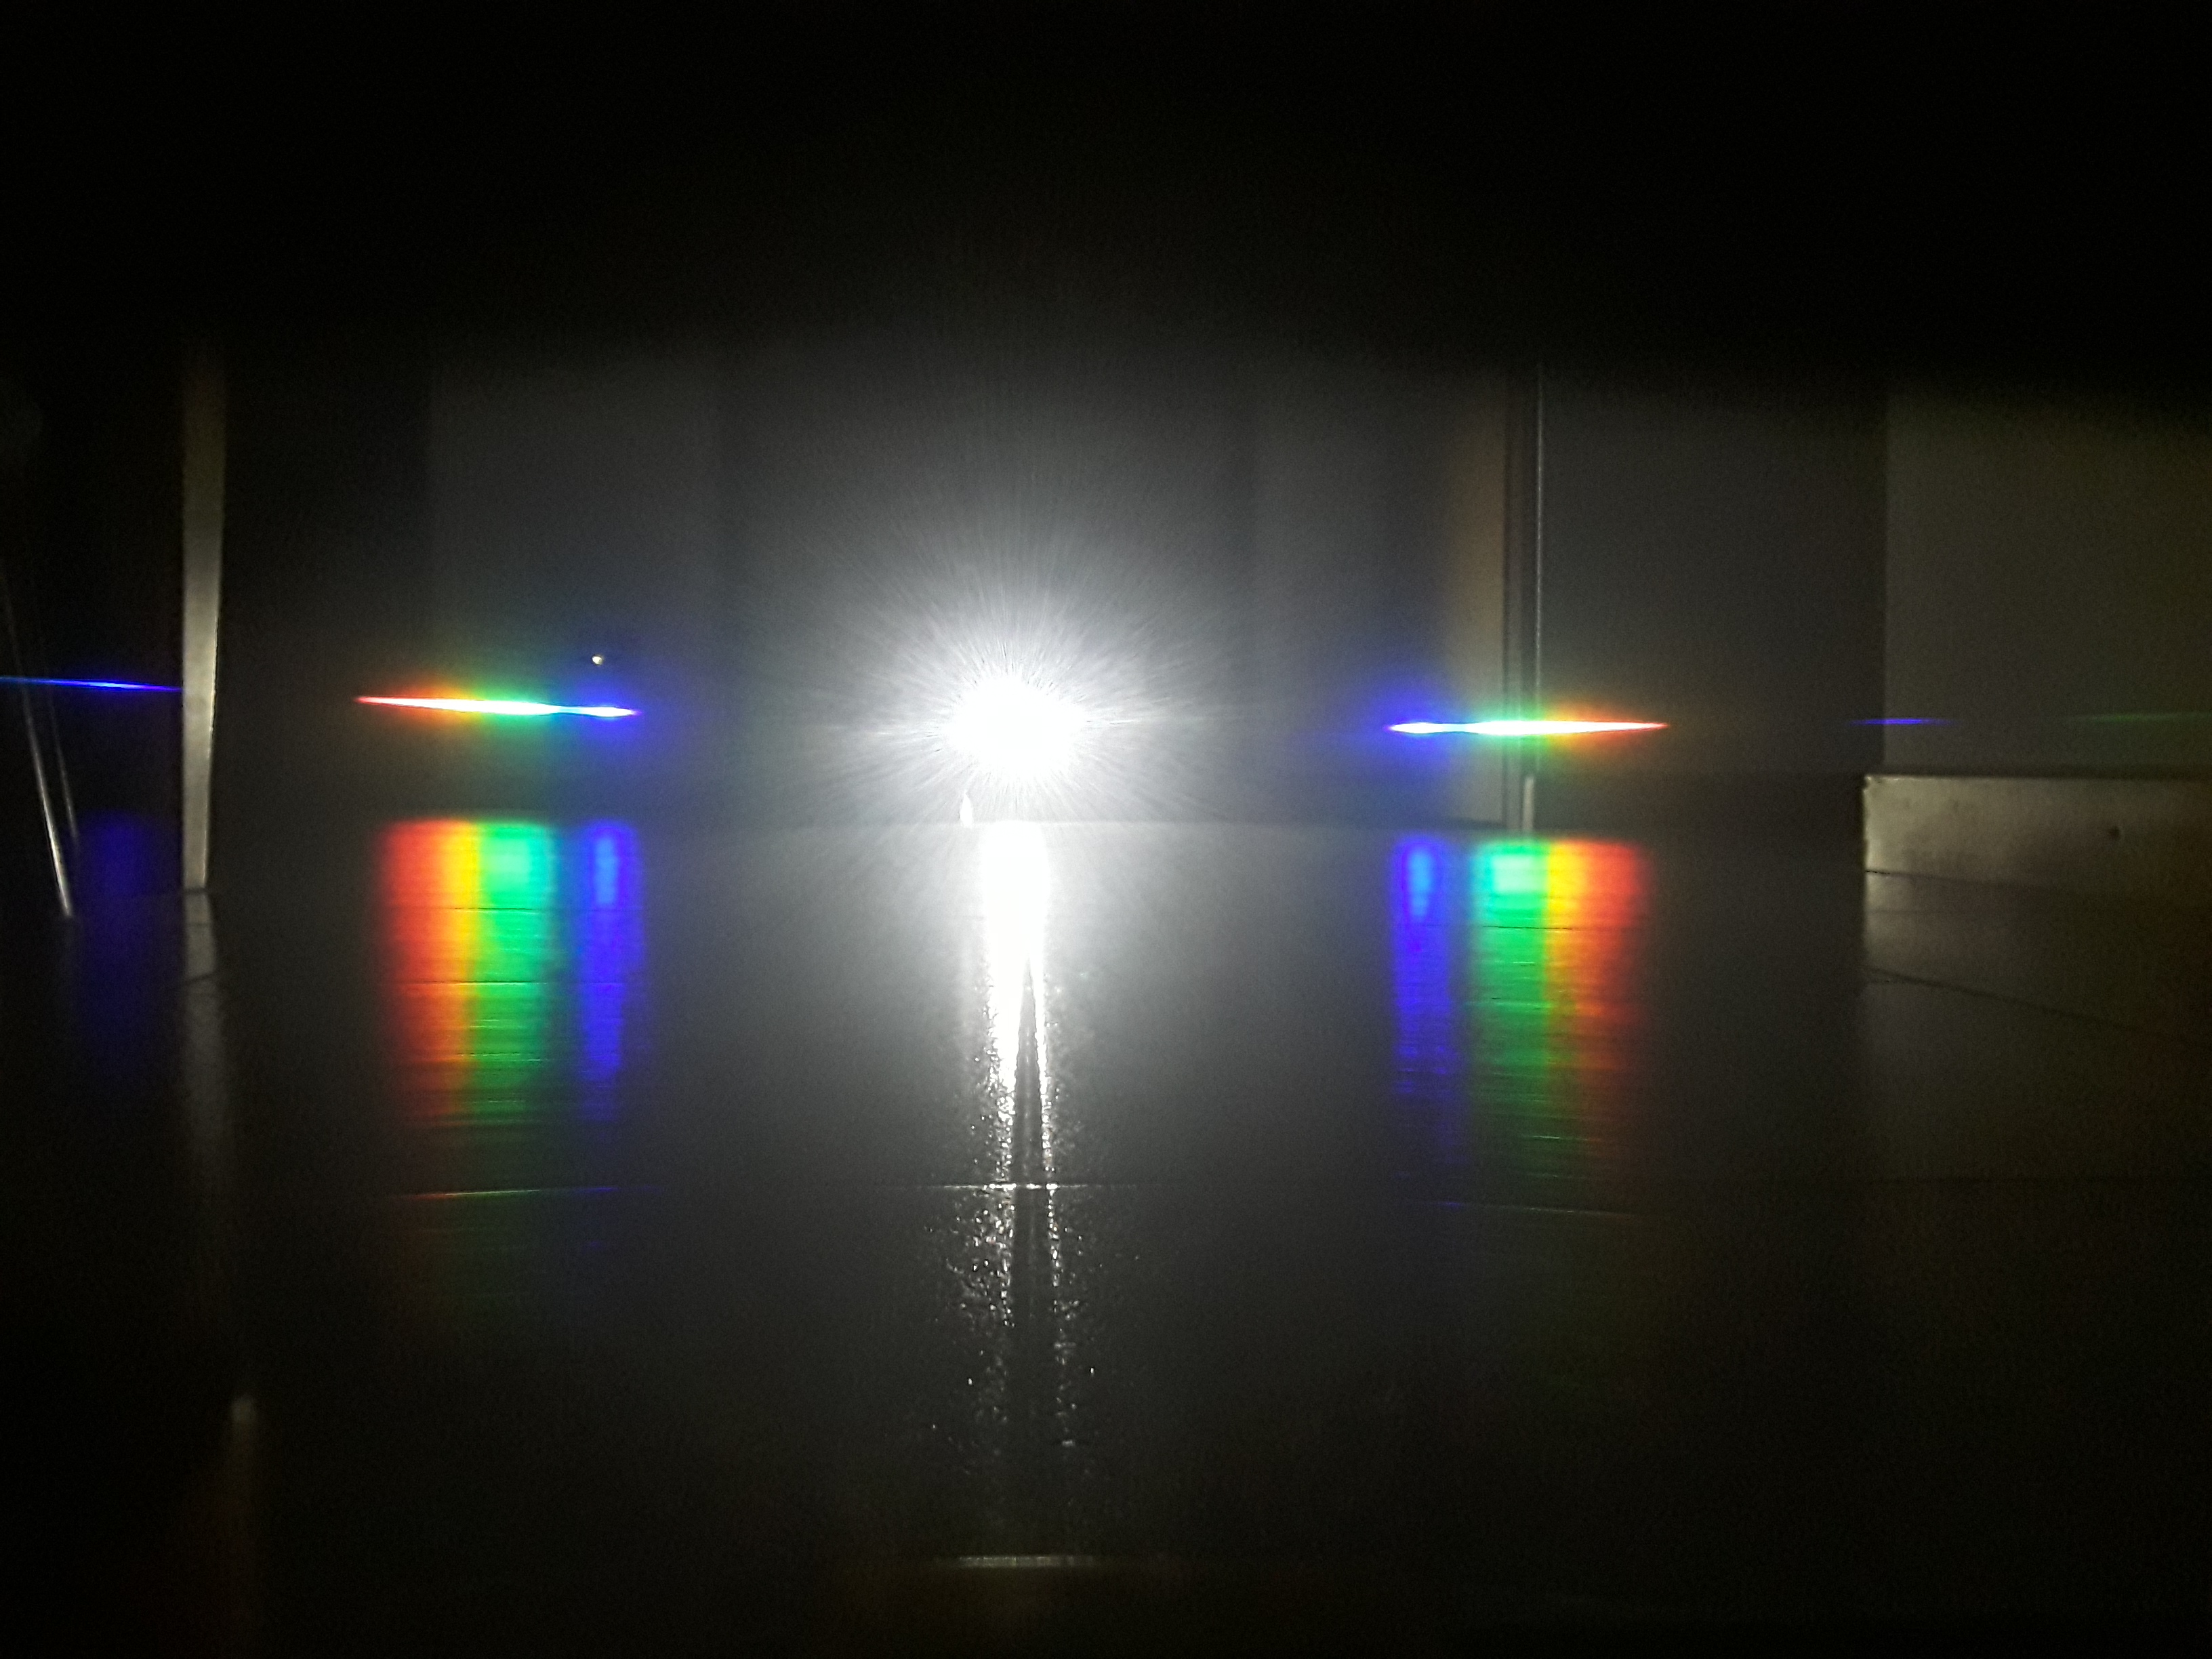
\includegraphics[width=0.6\linewidth]{IM 1.1.2}
  \caption{Foto della sorgente e dell'immagine diffratta (3.1, 3m)}
\end{figure}

\begin{figure}[h!]
  \centering
  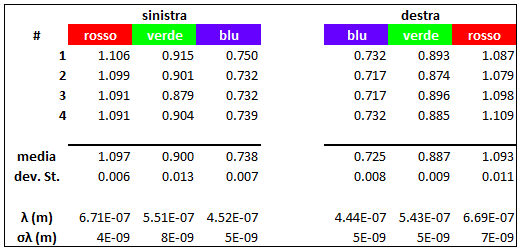
\includegraphics[width=0.6\linewidth]{IM tab_1.1.2}
  \caption{$\Delta x$ misurati (3.1, 3m)}
\end{figure}

\pagebreak

\subsection{lampada 1, reticolo passo ignoto}

Sostituito il reticolo di passo noto con quello di passo ignoto, è stata ripetuta la procedura descritta nella sezione precedente. Il fattore di correzione tiene conto solo del portapenne. I valori di $\lambda$ utilizzati sono quelli calcolati nella sezione Analisi dati. Le formule utilizzate sono

\[d = \frac{\lambda \cdot z}{\Delta x} \quad \quad \quad \sigma d = \sqrt{\left( \frac{z}{\Delta x} \sigma \lambda \right)^2 + \left( \frac{d \cdot \Delta x}{z^2}\sigma z \right)^2}\]

\begin{table}[h!]
\centering
\begin{tabular}{ | c | c | }
  \hline
  $\#$ & $z (m)$ \\
  \hline
  $1$ & $3,561$ \\
  $2$ & $3,561$ \\
  $3$ & $3,560$ \\
  $4$ & $3,559$ \\
  $5$ & $3,561$ \\
  $6$ & $3,560$ \\
  $7$ & $3,560$ \\
  $8$ & $3,555$ \\
  \hline 
  media & $3,560$ \\
  st. dev. & $0,002$ \\
  \hline
  $z$ (m) & $3,600$ \\
  $\sigma z$ (m) & $0,002$ \\
  \hline
\end{tabular}
\caption{Misura di $z$ (3.2)}
\end{table}

\begin{figure}[h!]
  \centering
  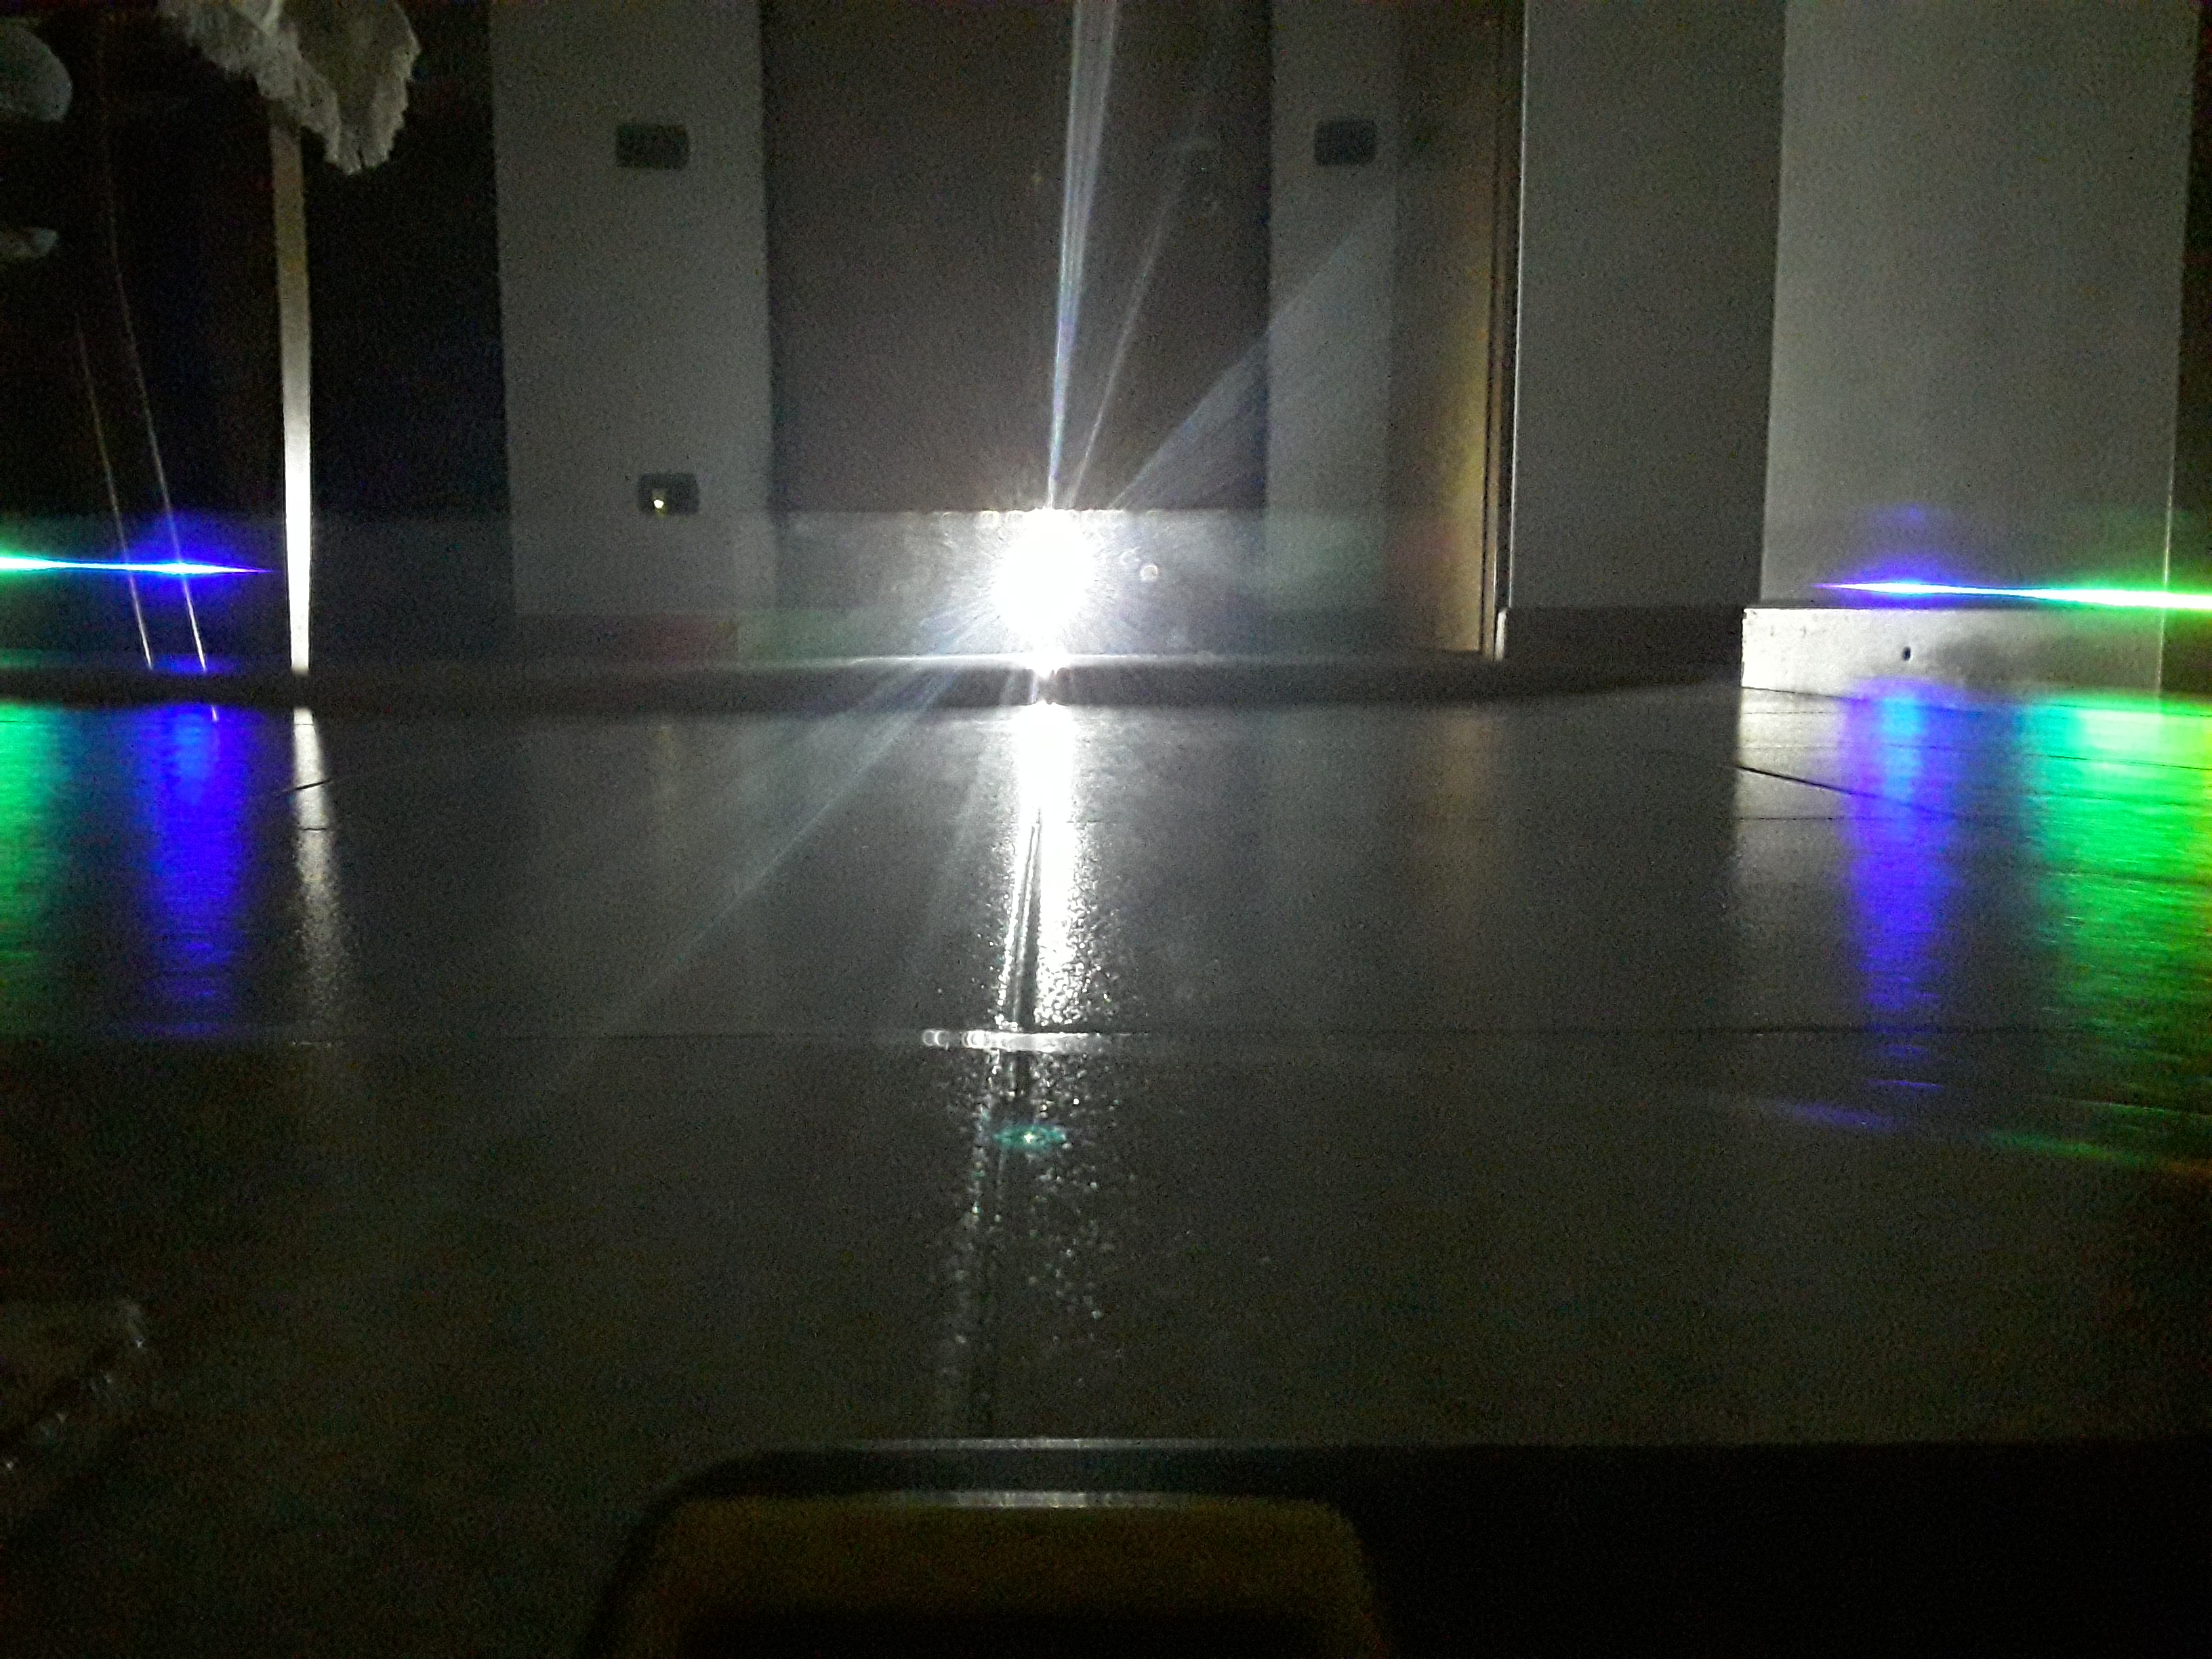
\includegraphics[width=0.6\linewidth]{IM 1.2}
  \caption{Foto della sorgente e dell'immagine diffratta (3.2)}
\end{figure}

\begin{figure}[h!]
  \centering
  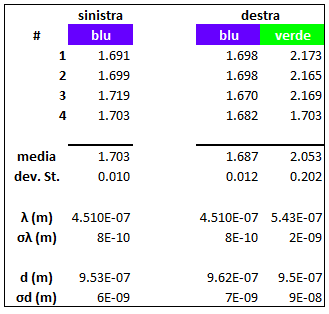
\includegraphics[width=0.4\linewidth]{IM tab_1.2}
  \caption{$\Delta x$ misurati (3.2)}
\end{figure}

\pagebreak

\subsection{lampada 2, reticolo passo noto}

Le procedure per la seconda lampada sono analoghe a quelle delle sezioni precedenti. Le misure di $z$ si sono svolte lo stesso giorno per entrambi i reticoli, quindi condividono la misura di $z$. Il fattore di correzione, per questa misura, è di $1$ cm, ed è dovuto allo spessore di uno schermo posto di fronte alla lampada, essendo questa troppo piccola per poter essere accuratamente centrata con il metro laser.

\begin{table}[h!]
\centering
\begin{tabular}{ | c | c | }
  \hline
  $\#$ & $z (m)$ \\
  \hline
  $1$ & $3,555$ \\
  $2$ & $3,555$ \\
  $3$ & $3,555$ \\
  $4$ & $3,555$ \\
  $5$ & $3,554$ \\
  $6$ & $3,555$ \\
  $7$ & $3,554$ \\
  $8$ & $3,554$ \\
  \hline 
  media & $3,555$ \\
  st. dev. & $0,002$ \\
  \hline
  $z$ (m) & $3,565$ \\
  $\sigma z$ (m) & $0,002$ \\
  \hline
\end{tabular}
\caption{Misura di $z$ (3.3)}
\end{table}

\begin{figure}[h!]
  \centering
  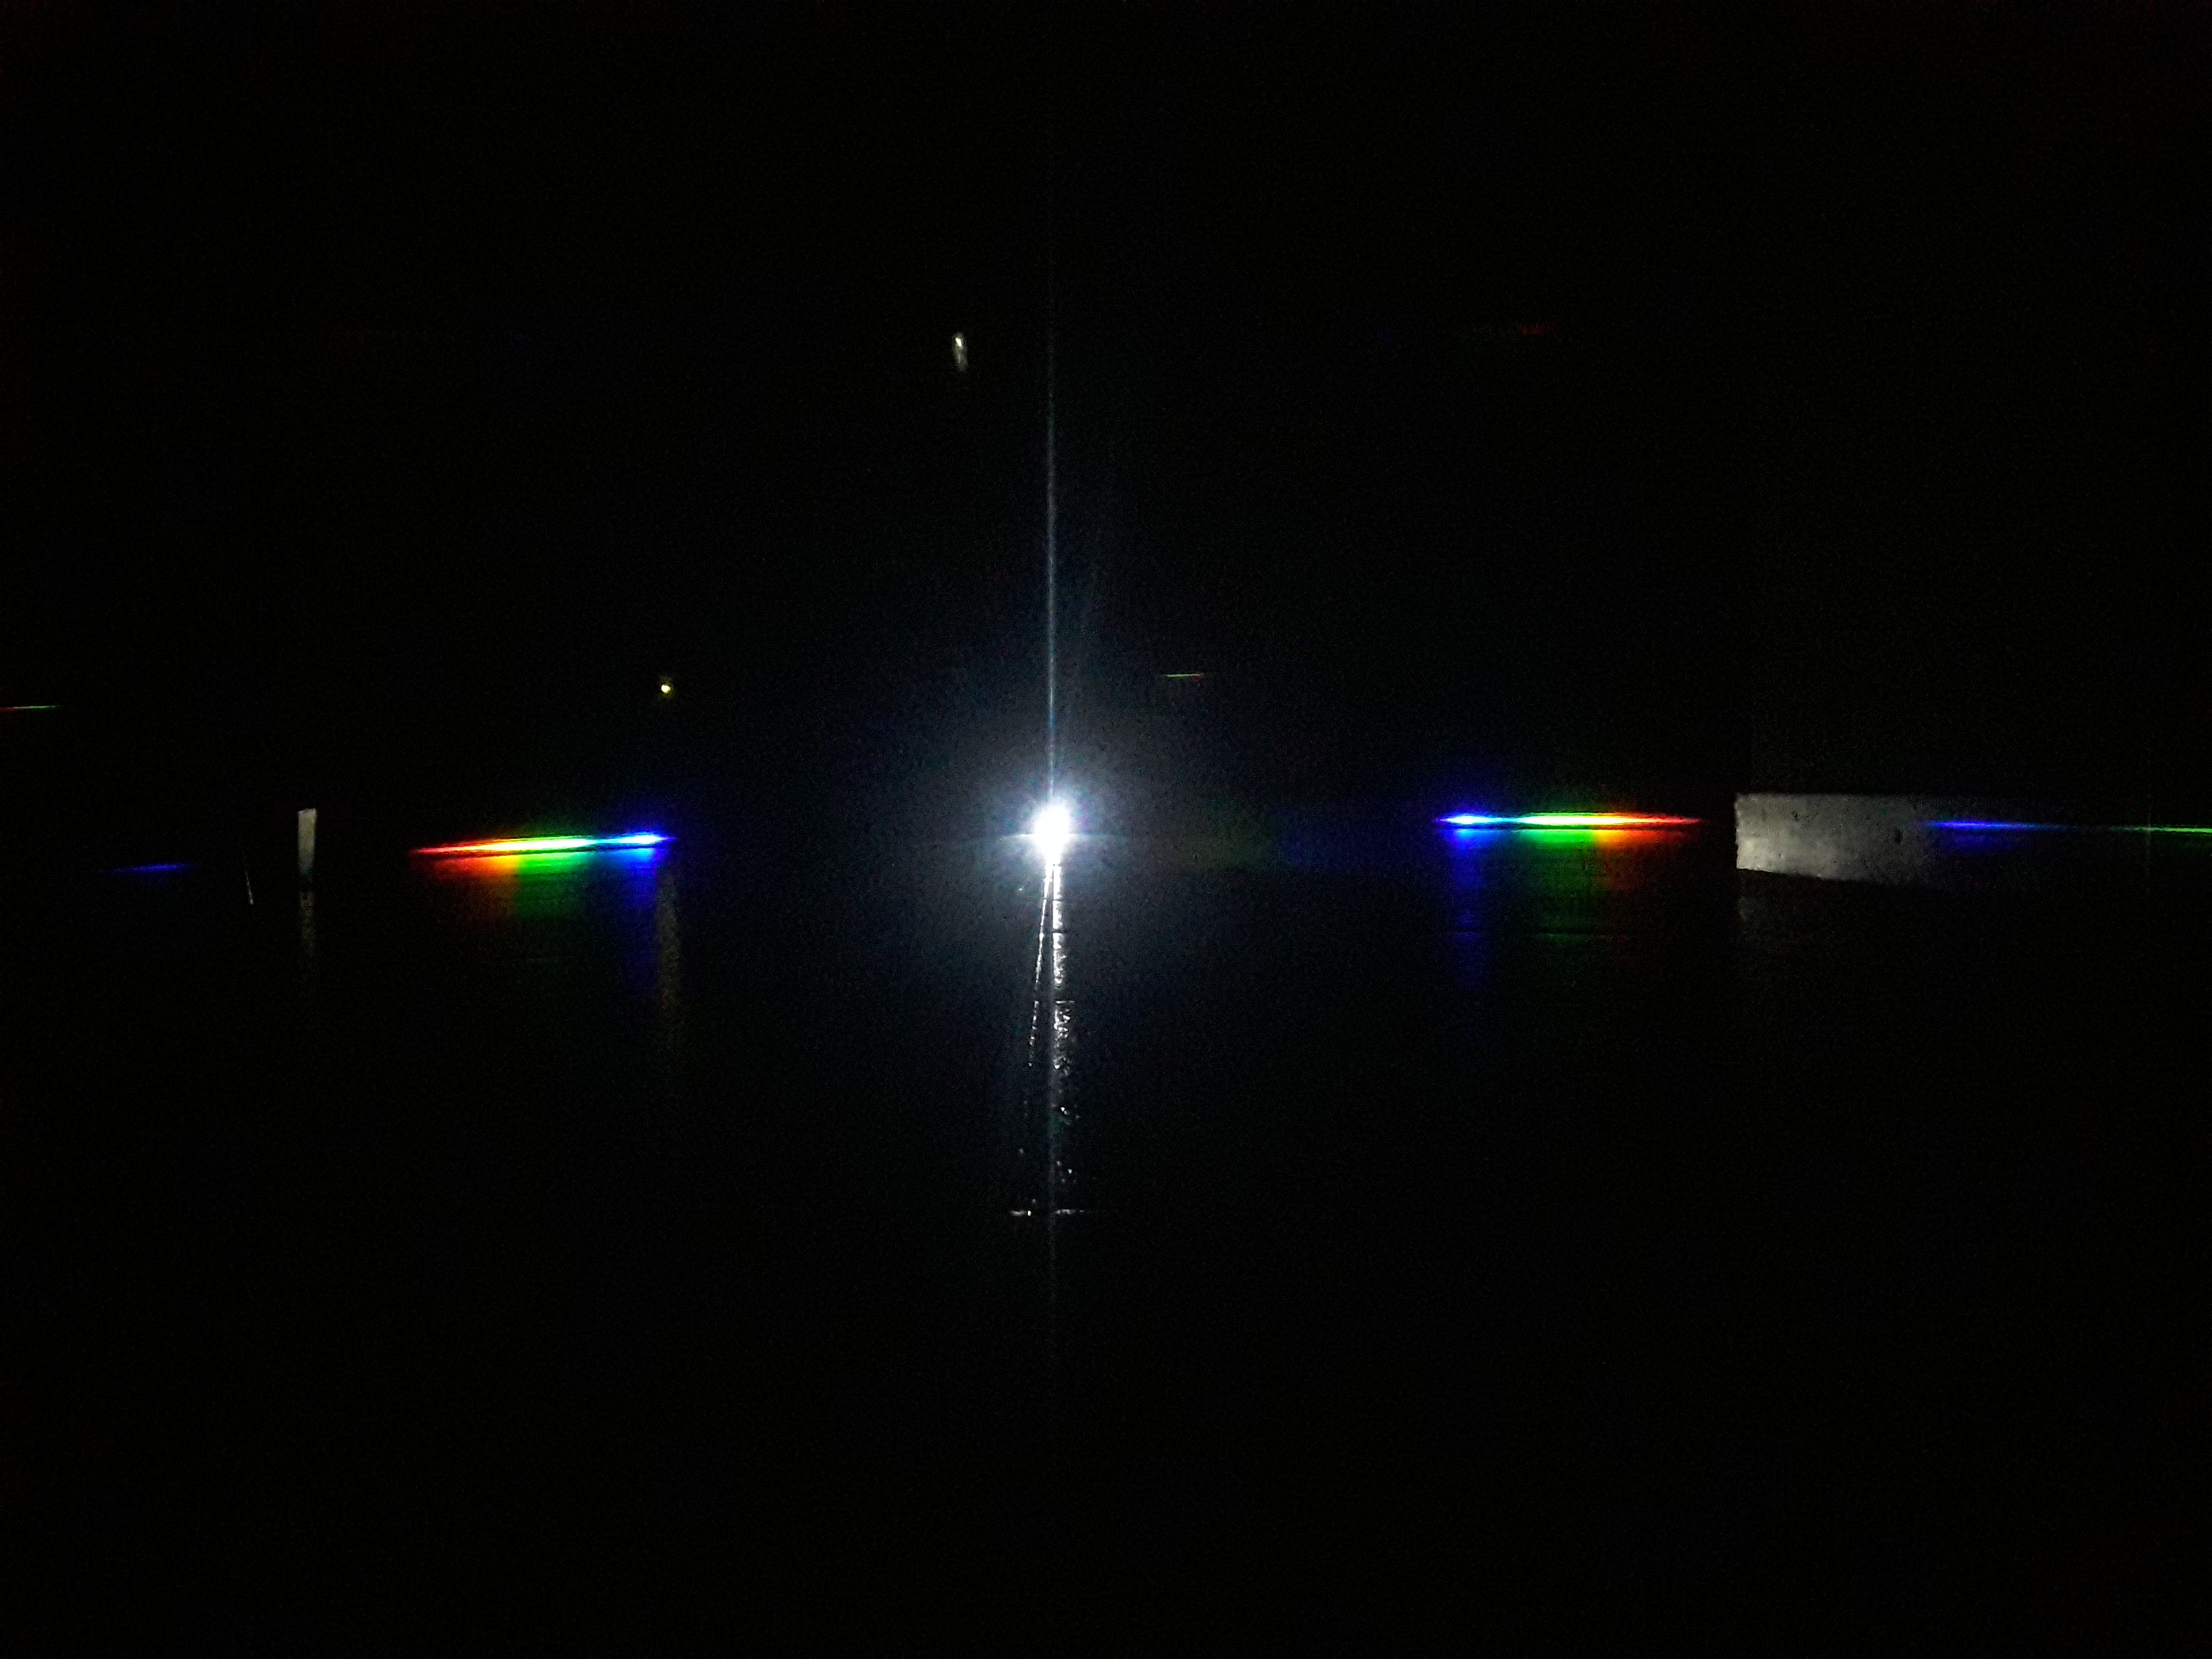
\includegraphics[width=0.6\linewidth]{IM 4.1}
  \caption{Foto della sorgente e dell'immagine diffratta (3.3)}
\end{figure}

\begin{figure}[h!]
  \centering
  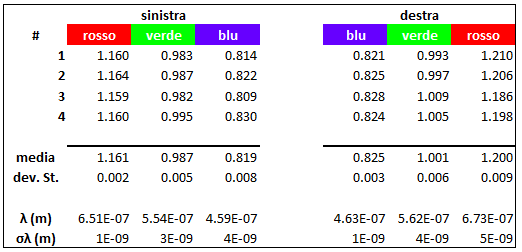
\includegraphics[width=0.6\linewidth]{IM tab_2.1}
  \caption{$\Delta x$ misurati (3.3)}
\end{figure}

\clearpage

\subsection{lampada 2, reticolo passo ignoto}

\begin{figure}[h!]
  \centering
  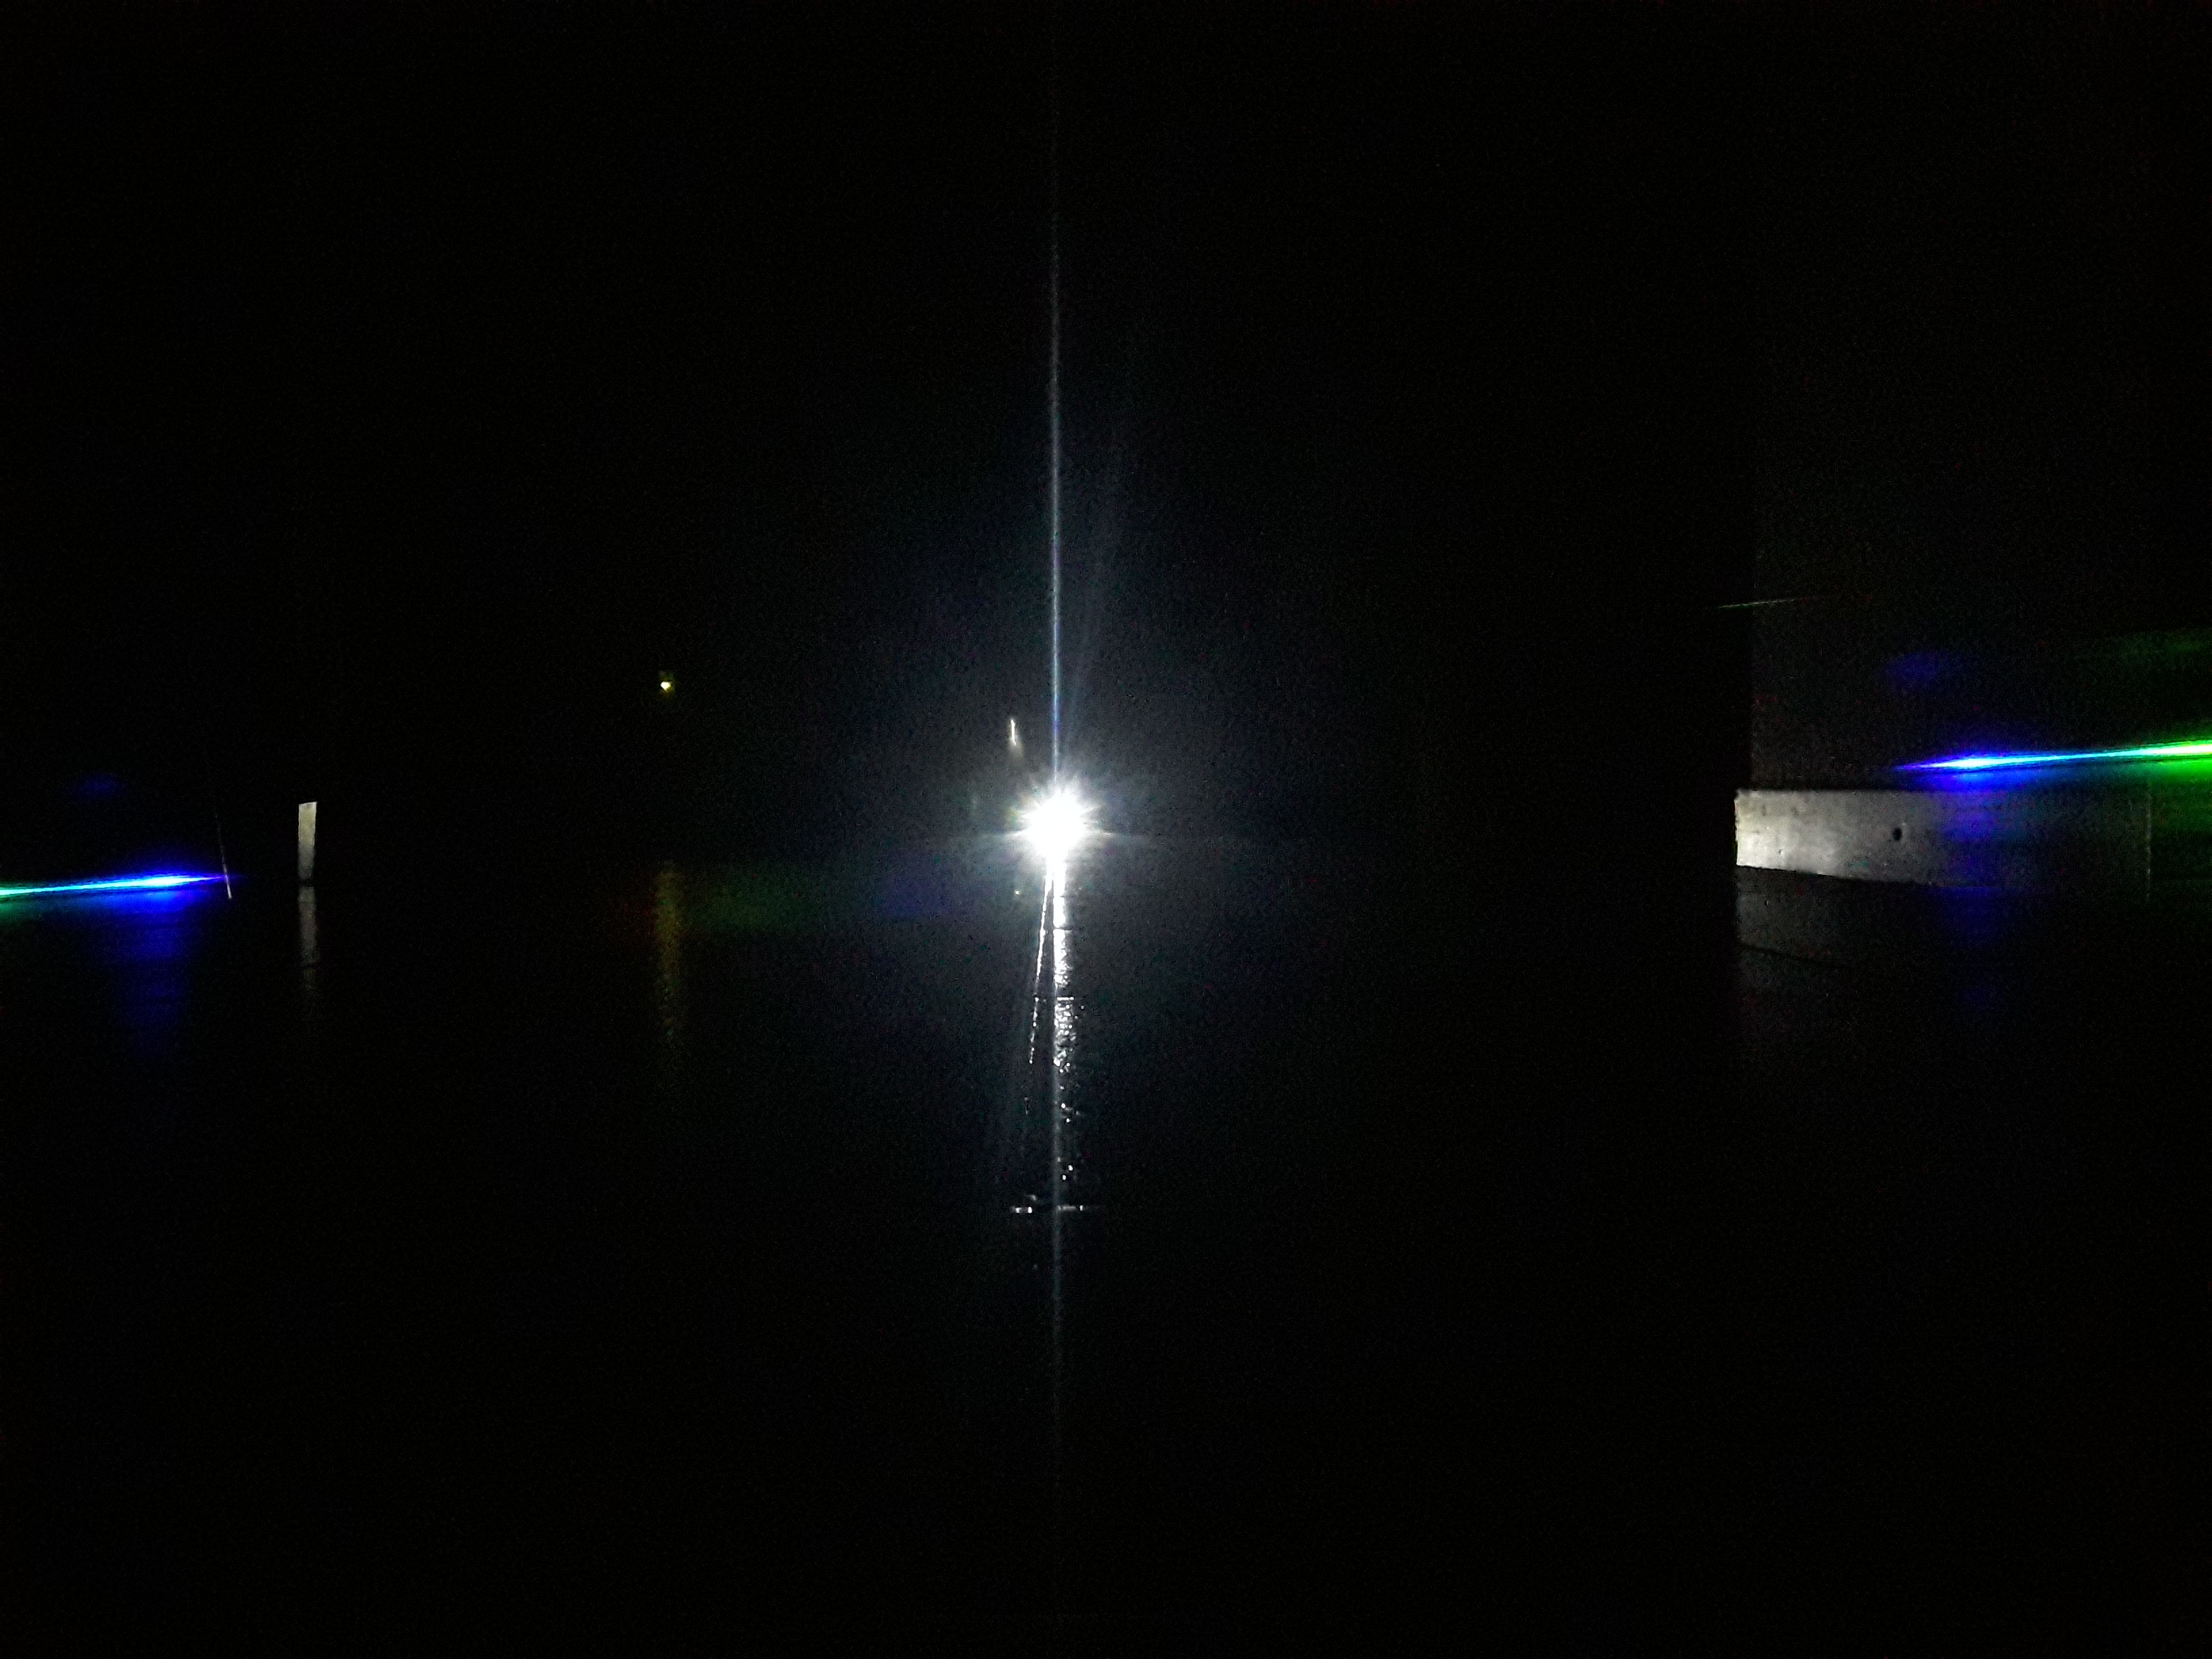
\includegraphics[width=0.6\linewidth]{IM 4.2}
  \caption{Foto della sorgente e dell'immagine diffratta (3.4)}
\end{figure}

\begin{figure}[h!]
  \centering
  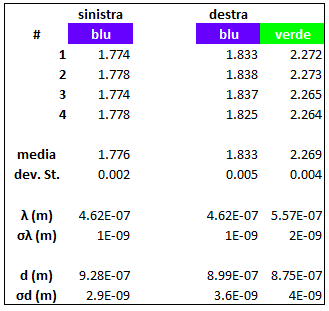
\includegraphics[width=0.4\linewidth]{IM tab_2.2}
  \caption{$\Delta x$ misurati (3.4)}
\end{figure}

\clearpage

\section{Analisi dati}

\subsection{lunghezze d'onda lampada 1}

È stata fatta una media pesata delle quantità misurate.

\begin{figure}[h!]
  \centering
  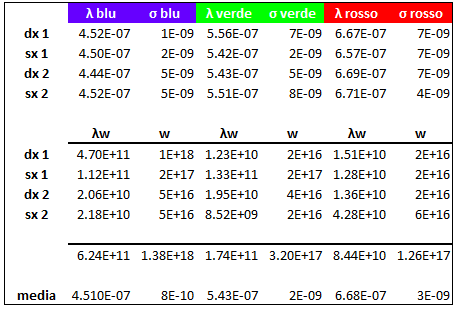
\includegraphics[width=0.6\linewidth]{IM tab_lambda_1}
  \caption{Medie pesate lambda lampada 1}
\end{figure}

\begin{figure}[h]
  \centering
  \begin{subfigure}[b]{0.3\linewidth}
    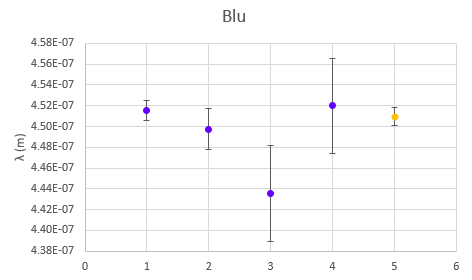
\includegraphics[width=\linewidth]{IM blu_lambda_1}
  \end{subfigure}
  \begin{subfigure}[b]{0.3\linewidth}
    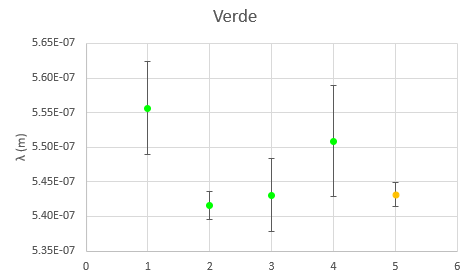
\includegraphics[width=\linewidth]{IM verde_lambda_1}
  \end{subfigure}
  \begin{subfigure}[b]{0.3\linewidth}
    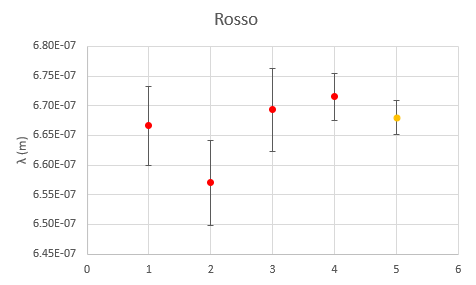
\includegraphics[width=\linewidth]{IM rosso_lambda_1}
  \end{subfigure}
  \caption{Grafici delle misure della lunghezza d'onda. In giallo la media pesata}
\end{figure}

Tutte le misure sono entro $2\sigma$ dalla media pesata. Considerando le condizioni non ottimali in cui è stata svolta la misura e le numerose approssimazioni effettuate, le ritengo accettabili.

\clearpage

\subsection{lunghezze d'onda lampada 2}

È stata fatta una media pesata delle lunghezze d'onda misurate.

\begin{figure}[h!]
  \centering
  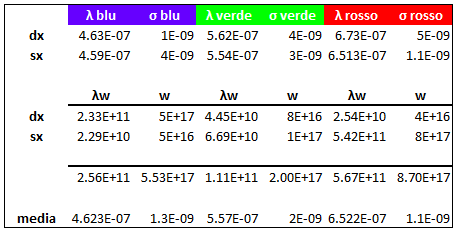
\includegraphics[width=0.6\linewidth]{IM tab_lambda_2}
  \caption{Medie pesate lambda lampada 2}
\end{figure}

\begin{figure}[h]
  \centering
  \begin{subfigure}[b]{0.3\linewidth}
    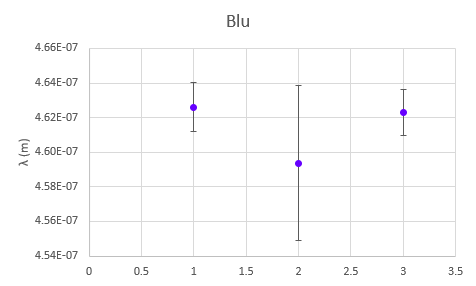
\includegraphics[width=\linewidth]{IM blu_lambda_2}
  \end{subfigure}
  \begin{subfigure}[b]{0.3\linewidth}
    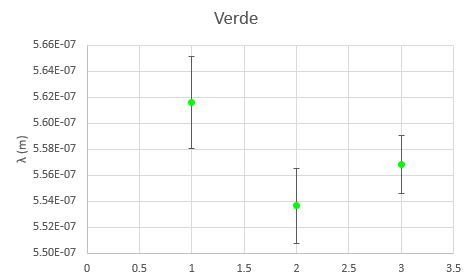
\includegraphics[width=\linewidth]{IM verde_lambda_2}
  \end{subfigure}
  \begin{subfigure}[b]{0.3\linewidth}
    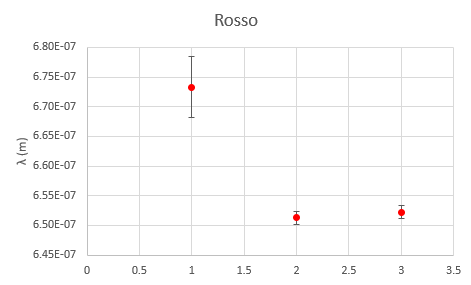
\includegraphics[width=\linewidth]{IM rosso_lambda_2}
  \end{subfigure}
  \caption{Grafici delle misure della lunghezza d'onda. Il terzo valore è la media pesata}
\end{figure}

Mentre le lunghezze d'onda misurate del blu e del verde sono compatibili tra di loro, quelle del rosso chiaramente non lo sono. Non avendo tempo di rifare la misura, l'ho scartata.

\clearpage

\subsection{Passo}

\begin{figure}[h!]
  \centering
  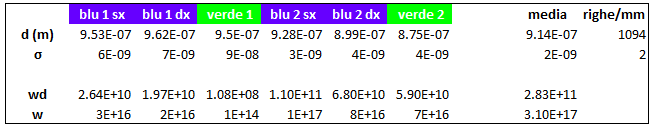
\includegraphics[width=0.6\linewidth]{IM_d}
  \caption{Media pesata del passo del reticolo}
\end{figure}

\begin{figure}[h!]
  \centering
  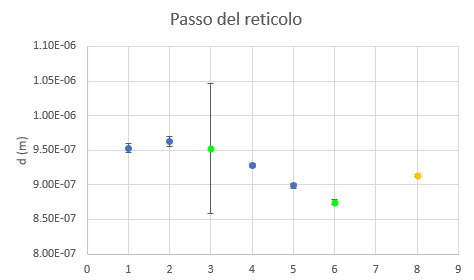
\includegraphics[width=0.6\linewidth]{IM grafico_d}
  \caption{Grafico delle misure del passo del reticolo. In giallo la media pesata}
\end{figure}

In questa misura emerge fortemente il problema dell'uso della deviaizone standard come incertezza. Le misure di $\Delta x$ sono state eseguite usando come riferimento il centro della sorgente luminosa e il centro dell'immagine. Il problema con questo modo di procedere è che si ottengono misure molto precise e con una devizione standard molto piccola, e mentre questo modo di procedere si è rivelato efficace per le misure delle lunghezze d'onda, per la misura del passo si ottengono delle incertezze decisamente troppo piccole.

Ho deciso quindi di trascurare l'incertezza strumentale e fare una semplice media aritmetica, e usare la deviazione standard della media come incertezza della mia stima del passo.

\begin{figure}[h!]
  \centering
  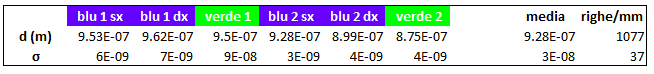
\includegraphics[width=0.6\linewidth]{IM_d_megl}
  \caption{Media del passo del reticolo}
\end{figure}

\begin{figure}[h!]
  \centering
  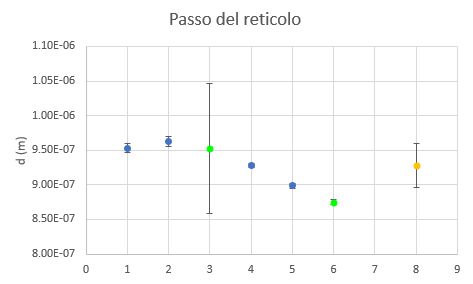
\includegraphics[width=0.6\linewidth]{IM grafico_d_megl}
  \caption{Grafico delle misure del passo del reticolo. In giallo la media}
\end{figure}

La mia miglior stima del passo del reticolo è

\[9,3 \cdot 10^{-7} \pm 3 \cdot 10^{-8} \; \textrm{m}\]

In termini di densità:

\[1077 \pm 37 \; \textrm{righe}/\textrm{mm}\]

\section{Conclusioni}

I valori delle lunghezze d'onda misurate sono coerenti con i colori osservati. La stima del passo del reticolo fornisce un valore che è circa metà di quello del reticolo di passo noto, coerente con la posizione osservata dell'immagine diffratta, il cui primo ordine cade all'incirca in corrispondenza del secondo ordine osservato con il reticolo di passo noto. 

La procedura sperimentale utilizzata potrebbe tuttavia aver portato ad una significativa sottostima delle incertezze.

\vspace{5mm}

L'esperimento può dirsi concluso con risultati accettabili.

\end{document}